\newpage
\section{Literature Review and Theory}
\subsection{Definition of Misinformation}

Misinformation encompasses a variety of different types of information, all of which have in common that they are false or misleading. It is spread predominantly via the internet and has become increasingly important through the rise of social media. According to Alessandro Bondielli et al., "fake news" and "rumors" are the types most commonly recognized as misinformation within public discourse. It is important to note, however, that the term also includes clickbait, social spam, and fake reviews. All of these elements can significantly impact societal decision-making by distorting the public's perception \cite{mi_alessandro_bondielli}. 

\begin{figure}[h]
    \centering
    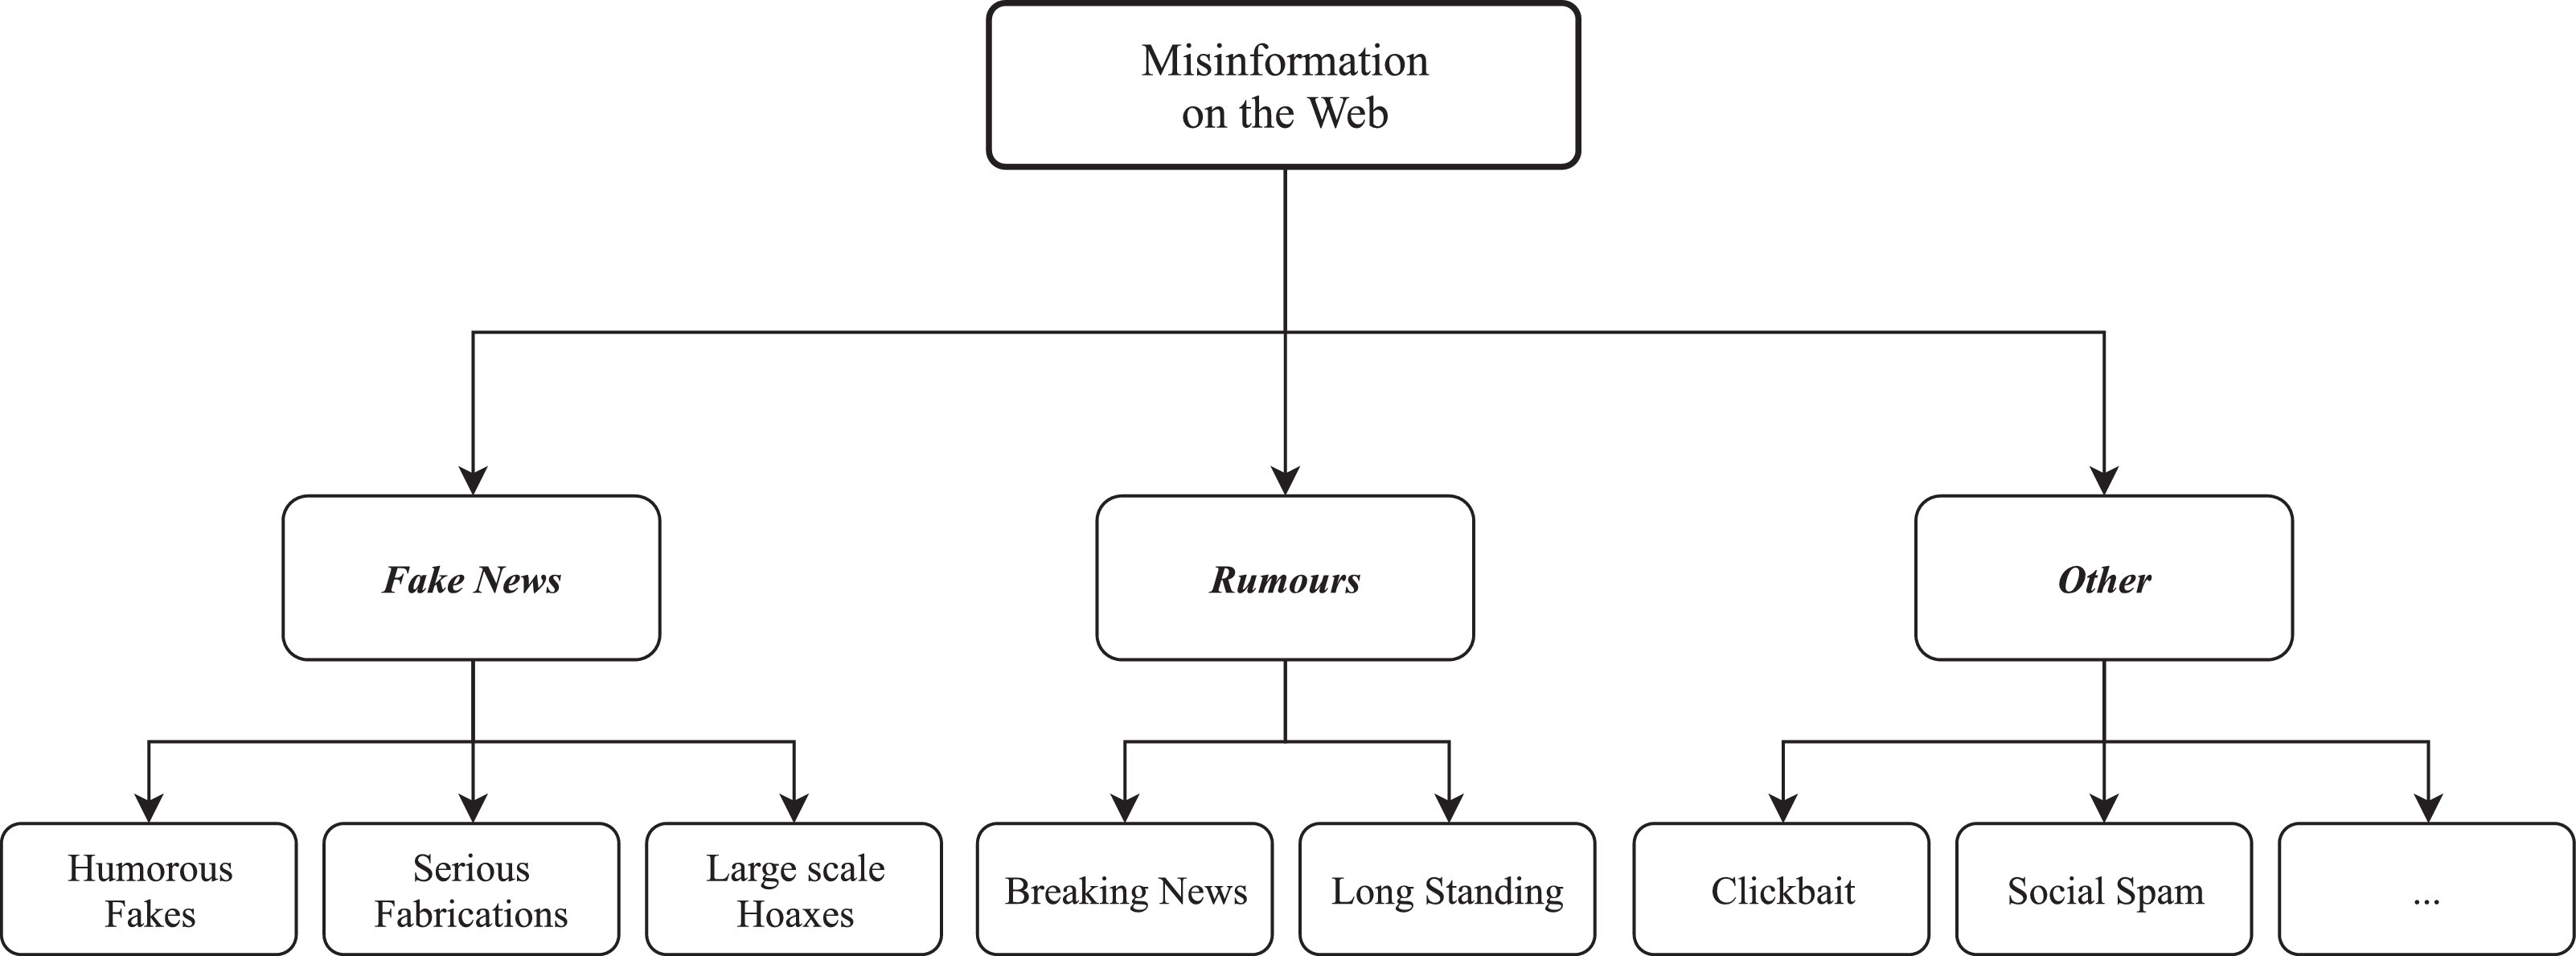
\includegraphics[width=1\textwidth]{assets/Types_Of_MisInformation.jpg}
    \caption{Different types of misinformation on the internet \cite{mi_alessandro_bondielli}.}
    \label{fig:my_label}
\end{figure}

Misinformation is often not spread accidentally. Fake news refers to content created with the explicit intent to deceive. Sometimes, one is only capable of disproving it through arduous verification processes. Rumors, on the other hand, are unverified pieces of information that may or may not be true but spread rapidly due to their sensational nature, especially on social platforms \cite{mi_alessandro_bondielli}.

In their study on Misinformation in Social Media, Liang Wu et al. expand this discussion by differentiating between misinformation and disinformation based on the originator's intent. According to them, disinformation is only a subset of misinformation which is created with the explicit intent to deceive. They emphasize, how in a social media environment, it can be difficult to discern if misinformation was created with intent or by accident. This makes the issue very complex for platform administrators and researchers alike. The Pizzagate incident, a conspiracy theory that ultimately led to a public shooting, is cited as an example of the potential consequences of misinformation \cite{mi_liang_wu}.

Md Rafiqul Islam et al. emphasize the intention behind misinformation, characterizing it as a means to create distrust within communities. They call for proactive measures in order to ensure the integrity of social discourse \cite{mi_rafiqul}. 

Trough platforms like Facebook or Twitter it has become far easier to spread misinformation. Misleading statements are frequently spread in conversations between individuals, where they are presented as factual. This can be particularly problematic in political contexts, where it may lead individuals who are misinformed to participate more actively and with more conviction in electoral processes than those who are uninformed \cite{mi_fernandez}.

In summary, misinformation is framed as a multifaceted problem that encompasses various types of incorrect or misleading information, each with individual origins and consequences. Addressing misinformation requires a nuanced approach that considers the intent behind the information, the medium through which it spreads, and the broader social context in which it exists.

\subsection{Misinformation Detection: From Traditional Methods to AI}
Traditionally, misinformation detection relied on manual verification by experts. However, the volume and velocity of online information are in need of an automated approach. Numerous researchers have developed systems as a means to detect and verify claims more efficiently. Most of those rely on advances made in \gls{ml} and \gls{nlp} \cite{claimbuster_arslan}.

There have been numerous studies on the application of \gls{ml} methods on misinformation detection \cite{MD_ML_1}\cite{MD_ML_2}\cite{MD_ML_3}\cite{MD_ML_4}. Early studies focus on more traditional \gls{ml} methods, mostly feature based modelling algorithms such as \gls{svm}, naive bayes or random forest classifiers. These are usually trained on lexical, n gram and sentiment features. Lexical features encompass measures such as number of words, average word length, count of numbers. 

The ngram feature is .. %TODO finish


\subsection{The Role of Deep Learning}

\subsubsection{Neural Networks in Detection}
While traditional \gls{ml} algorithms can provide high prediction accuracy, a number of recent studies have shown that deep learning models, especially advanced pre-trained language models deliver superior results in the detection of misinformation. 

\subsubsection{Advances in Transformer Models}
